%%%%%%%%%%%%%%%%%%%%%%%%%%%%%%%%%%%%%%%%%
%
% (c) 2019 by Jennifer Laaser
%
% This work is licensed under the Creative Commons Attribution-NonCommercial-ShareAlike 4.0 International License. To view a copy of this license, visit http://creativecommons.org/licenses/by-nc-sa/4.0/ or send a letter to Creative Commons, PO Box 1866, Mountain View, CA 94042, USA.
%
% The current source for these materials is accessible on Github: https://github.com/jlaaser/pogil-polymers
%
%%%%%%%%%%%%%%%%%%%%%%%%%%%%%%%%%%%%%%%%%

\renewcommand{\figpath}{content/polymphys/mechanical-properties/viscoelasticity/figs}
\newcommand{\labelbase}{}
\renewcommand{\labelbase}{viscoelasticity}

\begin{activity}[Viscoelasticity of Polymeric Materials]

\begin{instructornotes}

	This activity introduces students to ...
	
	After completing this activity, students will be able to:
			\begin{enumerate}
				\item ...
			\end{enumerate}
	
			
	\subsection*{Activity summary:}
	\begin{itemize}
		\item \textbf{Activity type:} Learning Cycle
		\item \textbf{Content goals:} ...
		\item \textbf{Process goals:} %https://pogil.org/uploads/attachments/cj54b5yts006cklx4hh758htf-process-skills-official-pogil-list-2015-original.pdf
			written communication, critical thinking, information processing
		\item \textbf{Duration:} TBD %approx. 45 minutes without class discussion
		\item \textbf{Instructor preparation required:} 
			\begin{itemize}
				\item Prepare small samples of silly putty (or comparable silicone putty) for each student group
			\end{itemize}
		\item \textbf{Related textbook chapters:}
			\begin{itemize}
				\item \emph{Polymer Chemistry} (Hiemenz \& Lodge): ...
			\end{itemize}
	\end{itemize}

\end{instructornotes}

	%\textbf{Focus question:} Put a central question for the students to consider through this exercise here.

\begin{model}[Properties of Silicone Putty]
\label{model:sillyputty}

	Obtain a small sample of silicone putty from your instructor.
	
	Do the following experiments, and note your observations about how the material responds:
	
	\begin{enumerate}
		\item Place a small ball of putty on a table, and hit it quickly with your hand.
			\begin{itemize}
				\item Observations:
				
				\begin{solution}[0.75in]
				
					The putty mostly retains its shape.
					
				\end{solution}
			\end{itemize}
		
		\item Place a small ball of putty on your desk, and let it sit without touching it for 1-2 minutes.
			\begin{itemize}
				\item Observations:
				
				\begin{solution}[0.75in]
				
					The putty initially retains its shape, but over time, slowly begins to flow and flatten out.
					
				\end{solution}
			\end{itemize}
		
		\item Take a small piece of putty and stretch it between your hands.  Vary the rate at which you stretch it (quickly vs. slowly).
			\begin{itemize}
				\item Observations:
				
				\begin{solution}[1in]
				
					When the putty is pulled slowly, it stretches like taffy.
					
					When the putty is pulled quickly, it may break.
					
				\end{solution}
			\end{itemize}
		
	\end{enumerate}

\end{model}


\begin{ctqs}

	\question In which of your experiments would you say the putty behaved more like an \emph{elastic solid}?  Briefly explain your reasoning.
	
		\begin{solution}[1.25in]
		
			In experiment (1), the putty retains its shape, and is thus more solid-like.
			
			In experiment (3), when pulled quickly, the putty ``breaks'', which is also a solid-like behavior.
		
		\end{solution}
	
	\question In which of your experiments would you say the putty behaved more like a \emph{viscous liquid}?  Briefly explain your reasoning.
	
		\begin{solution}[1in]
		
			In experiment (2), the putty flowed to match the shape of the surface it was sitting on, which is a liquid-like behavior.
		
		\end{solution}
	
	\question How did your observation of solid-like or liquid-like properties depend on the rate of deformation (i.e. how quickly you deformed or manipulated the putty)?
	
		\begin{solution}[1in]
		
			When the rate of deformation was high, the putty behaved more like a solid.
			
			When the rate of deformation was low, the putty behaved more like a liquid.
			
		\end{solution}
		
	\question Explain, in one or two complete sentences, why you think we might describe this putty as a ``viscoelastic'' material.
	
			\begin{solution}[1.5in]
			
				We describe this putty as a viscoelastic material because it  has some properties of both elastic solids (elasticity, ability to hold its shape) and of viscous liquids (ability to flow).  The properties that we observe depend on the timescale of the observation.
				
			\end{solution}
		
\end{ctqs}

\begin{model}[Step-Strain Experiments on Liquids and Solids]

	explain a step-strain experiment
	
\end{model}

\begin{ctqs}
	\question WALK STUDENTS THROUGH ELASTIC SOLID (BY ANALOGY TO RUBBER BAND)
	
	\question  WALK STUDENTS THROUGH VISCOUS LIQUID (BY ANALOGY TO MOVING HAND THROUGH WATER)
	
\end{ctqs}

\begin{infobox}

	Solid-like materials are typically described in terms of their \emph{modulus}, E (for extensional strain) or G (for shear strain).  For an elastic solid subjected to a strain of size $\epsilon$ (for extensional strain) or $\gamma$ (for shear strain), the resulting stress, $\sigma$, is directly proportional to the strain:
	\begin{align*}
		\sigma &= E\epsilon\,\,\,\,\,\,\,\text{(extensional strain)}\\
		%&\text{or}\\
		\text{or}\,\,\,\,\,\,\sigma &= G\gamma\,\,\,\,\,\,\,\text{(shear strain)}
	\end{align*}
	
	Liquid-like materials are typically described in terms of their \emph{viscosity}, $\eta$.  For a liquid, the stress is proportional to the strain \emph{rate}:
	\begin{align*}
		\sigma &= \eta\frac{d\epsilon}{dt}=\eta\dot\epsilon\,\,\,\,\,\,\,\text{(extensional strain)}\\
		%&\text{or}\\
		\text{or}\,\,\,\,\,\,\sigma &= \eta\frac{d\gamma}{dt}=\eta\dot\gamma\,\,\,\,\,\,\,\text{(shear strain)}
	\end{align*}

\end{infobox}

\begin{ctqs}
	\question PLOT STRESS PROFILES FOR STEP-STRAIN
	
	\question ARE THEY CONSISTENT WITH PREDICTIONS?
\end{ctqs}
	

\begin{model}[The Maxwell Model]
\label{\labelbase:mdl:maxwell}

	One of the simplest models we can use to describe viscoelasticity of polymeric materials is the \emph{Maxwell model}.
	
	In this model, we imagine the response of the material as being represented by a spring \emph{and} a dashpot, connected in series:
	
	\centerline{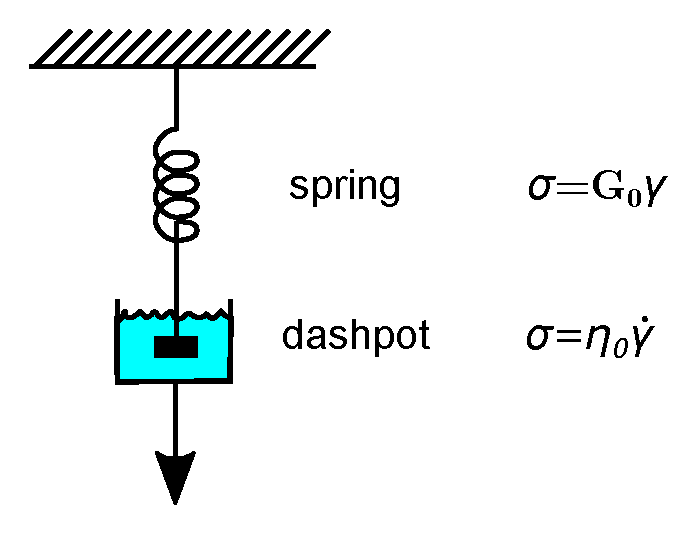
\includegraphics[width=0.5\textwidth]{\figpath/model2-maxwellelement}}
	
\end{model}

	
\begin{ctqs}
	\question (GET THEM TO REASON THROUGH EXPONENTIAL DECAY)
	
					\begin{solution}[2.5in]
					\end{solution}
					
\end{ctqs}

\begin{infobox}
	As shown in Exercise \ref{\labelbase:exc:maxwell}, the time-dependent stress for a step-strain experiment on the Maxwell model works out to be:
	\begin{align*}
		\sigma(t) = \sigma_0 e^{-t G_0/\eta_0}  && \text{or} && \sigma(t) = \sigma_0 e^{-t /\tau}
	\end{align*}
	where $\tau = \eta_0/G_0$.
\end{infobox}

\begin{ctqs}
	
	\question Is this equation consistent with your prediction from question  NNN?  Why or why not?
	
					\begin{solution}[1.5in]
					\end{solution}
		
	\question At what time $t$ will $\sigma(t)$ drop to 1/e of its initial value?
	
					\begin{solution}[1.5in]
					\end{solution}
		
		\question Why might we refer to $\tau$ as the ``characteristic relaxation timescale''?  Explain your reasoning in 1-2 complete sentences.
	
					\begin{solution}[1.5in]
					\end{solution}
		
\end{ctqs}

\begin{model}[Small-Amplitude Oscillatory Shear Rheology]
\label{model:rheology}

	One of the most common experimental techniques used to characterize the viscoelasticity of polymeric materials is small-amplitude oscillatory shear rheology (SAOS).
	
	In a SAOS measurement, the sample is sandwiched between two surfaces that rotate back and forth at frequency $\omega$, resulting in a sinusoidally-varying strain:
	\begin{equation*}
		\gamma(t) = \gamma_0 \sin(\omega t)
	\end{equation*}
	
	The instrument (a rheometer) then measures the resulting force as a function of time, $\sigma(t)$, and breaks it down into two components: one that is proportional to $\sin(\omega t)$ and one that is proportional to $\cos(\omega t)$. The response of the material can thus be expressed as follows:
	\begin{equation*}
		G(t) = \frac{\sigma(t)}{\gamma_0} = G' \sin(\omega t) + G'' \cos(\omega t)
	\end{equation*}

\end{model}

%\vspace{0.25in}
\begin{ctqs}
		
		\question In this experiment, the strain is proportional to $\sin(\omega t)$.  
			\begin{enumerate}
				\item Which coefficient, $G'$ or $G''$, tells you how much of the response is directly proportional to the applied strain?
	
					\begin{solution}[1in]
						$G'$ is in the term that goes as $\sin(\omega t)$, so $G'$ is the coefficient that tells us how much of the response is directly proportional to the applied strain.
					\end{solution}
		
		\item Does this coefficient tell you about the elastic response of the material, or the viscous response of the material?
	
					\begin{solution}[1in]
						The elastic response is directly proportional to the applied strain, so this coefficient tells us about the elastic response.
					\end{solution}
					
			\end{enumerate}
			
		\question Since $\frac{d}{dt}\sin(\omega t) \sim \cos(\omega t)$, the strain \emph{rate} in this experiment is proportional to $\cos(\omega t)$.
		
			\begin{enumerate}
		
				\item Which coefficient, $G'$ or $G''$, tells you how much of the response is proportional to the strain rate?
	
					\begin{solution}[1in]
						The $G''$ term is proportional to $\cos(\omega t)$, so $G''$ tells us about the portion of the response that is proportional to strain rate.
					\end{solution}
		
				\item Does this coefficient tell you about the elastic response of the material, or the viscous response of the material?
	
					\begin{solution}[1in]
					
						The viscous response is proportional to the strain rate, so this coefficient tells us about the viscous repsonse.
					
					\end{solution}
					
			\end{enumerate}
		
		\question Remembering that elastic responses store energy, and viscous responses dissipate energy, explain why we call $G'$ the ``storage modulus'' and $G''$ the ``loss modulus'' of the material.
	
					\begin{solution}[2in]
					
						$G'$ gives information about the elastic response, which stores energy, so $G'$ is called the storage modulus.
						
						$G''$ gives information about the viscous response, which dissipates energy, so $G''$ is called the loss modulus.
					\end{solution}
			
\end{ctqs}

\begin{infobox}
	For the Maxwell model, the storage and loss moduli are given by:
	\begin{align*}
		G' = G_0 \frac{\omega^2 \tau^2}{\omega^2 \tau^2 + 1} && \text{and} && G'' = G_0 \frac{\omega \tau}{\omega^2 \tau^2 + 1}
	\end{align*}
	
\end{infobox}

\clearpage
\begin{ctqs}
	
	\question A plot of the storage and loss moduli as a function of frequency is shown below:
				
		\centerline{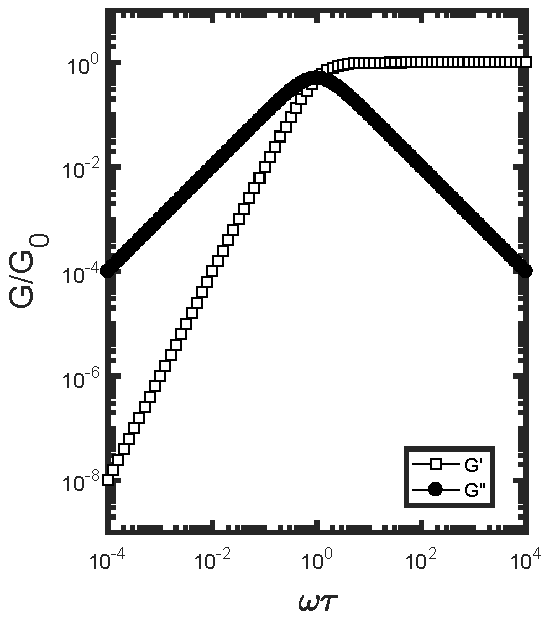
\includegraphics[width=0.4\textwidth]{\figpath/model3-maxwellplot}}
	
	Note that both axes of this graph are plotted on a log scale, and the x axis has been scaled by the characteristic relaxation time, $\tau$. 
	Using this graph, answer the following questions:
	
	\begin{enumerate}
		\item  At low frequencies (corresponding to long observation timescales), which is greater, the storage modulus or the loss modulus?  Is this consistent with your expectations?  Briefly explain your answer in 1-2 complete sentences.
	
					\begin{solution}[1.1in]
					
						At low frequencies, the loss modulus is greater.  This makes sense, because on long timescales, the material should be mostly liquid-like.
					
					\end{solution}
	
		\item At high frequencies (corresponding to short observation timescales), which is greater, the storage modulus or the loss modulus?  Is this consistent with your expectations?  Briefly explain your answer in 1-2 complete sentences.
	
					\begin{solution}[1.1in]
					
						At high frequencies, the storage modulus is greater.  This makes sense, because on long timescales, the material should be mostly solid-like.
					\end{solution}
	\end{enumerate}

	\question At what frequency is the storage modulus exactly equal to the loss modulus?  Give your answer in terms of the characteristic relaxation time, $\tau$.
	
		\emph{Note: you can answer this using either the graph or the equations, but you will probably find it easier to work from the equations.}
	
					\begin{solution}[1.75in]
					
						Setting the equations for $G'$ and $G''$ equal to each other, we have
						\begin{align*}
							G' &= G''\\
							G_0 \frac{\omega^2 \tau^2}{\omega^2 \tau^2 + 1} &= G_0 \frac{\omega \tau}{\omega^2 \tau^2 + 1}\\
							\omega^2 \tau^2 &= \omega \tau\\
							\omega\tau &= 1\\
							\omega &= \frac{1}{\tau}
						\end{align*}
					\end{solution}
	
	\question Rearrange your answer to the previous question to find an expression for the characteristic relaxation time in terms of the crossover frequency.
	
					\begin{solution}[1in]
					
						\begin{align*}
							\tau = \frac{1}{\omega_c}
						\end{align*}
					\end{solution}
	
	\question The following plot shows the dynamic moduli of a material similar to the silicone putty you experimented with at the beginning of this activity:
				
		\centerline{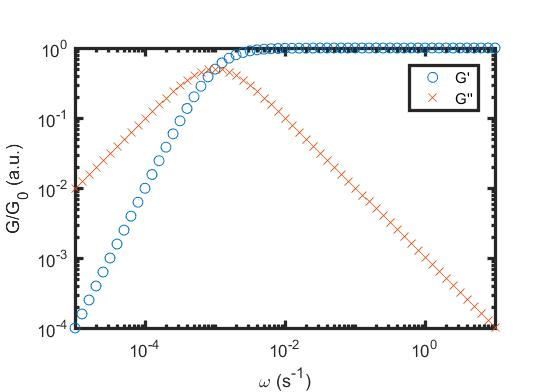
\includegraphics[width=0.6\textwidth]{\figpath/model3-maxwellexample.jpg}}
		
			Using this plot and your answer to the previous question, find the characteristic relaxation time of this polymer.
	
					\begin{solution}[1.5in]
					
						The storage and loss moduli are equal when $\omega=10^{-3}\text{ s}^{-1}$.  Thus the characteristic relaxation time is
						
						\begin{equation*}
							\tau = \frac{1}{\omega_c} = \frac{1}{10^{-3}\text{ s}^{-1}} = 1000\text{ s} \approx 17\text{ min}
						\end{equation*}
					\end{solution}
	
	\question If you were to pick up a sample of this polymer, would you expect it to feel more like a liquid or more like a solid?  Briefly justify your answer in 2-3 complete sentences.
	
		\emph{Hint: think about how the timescale on which you are observing/interacting with the polymer compares to the relaxation time!}
	
					\begin{solution}[2in]
					\end{solution}
	
\end{ctqs}
	

%\clearpage
\begin{exercises}

		\exercise Viscoelastic properties can arise from a number of molecular-scale interactions.  Which of the following do you think would give rise to viscoelastic properties in a polymeric material?  For each interaction that you think would cause a viscoelastic response, identify the physical process that you think would be most closely associated with the relaxation time of the material.
		
			\begin{enumerate}
				\item Covalent crosslinking of the polymer chains
				\item Hydrogen bonds (or other ``sticky'' noncovalent interactions) between polymer chains
				\item ``Tangling'' of long polymer chains around each other
			\end{enumerate}
			
		% exercise connecting to polymer processing? e.g. why is it important to control viscoelasticity in processing?
		
		\exercise In our discussion of the Maxwell Model, we considered a step-strain experiment, where we pulled the material to a set distance and then held it there.
		
			Another type of experiment we could conduct is a ``step-stress'' experiment, in which we simply begin pulling on the material with a constant force.  Make plots of (a) the applied stress and (b) the resulting strain that you would expect for this experiment.
			
		\exercise \label{\labelbase:exc:maxwell} DERIVE STEP-STRESS RESPONSE FOR MAXWELL MODEL
		
		\exercise The Maxwell Model is one simple model that yields viscoelastic behavior.  Another model that gives viscoelastic behavior is the Voigt model, in which the spring and dashpot are connected in parallel rather than in series:
		
			\centerline{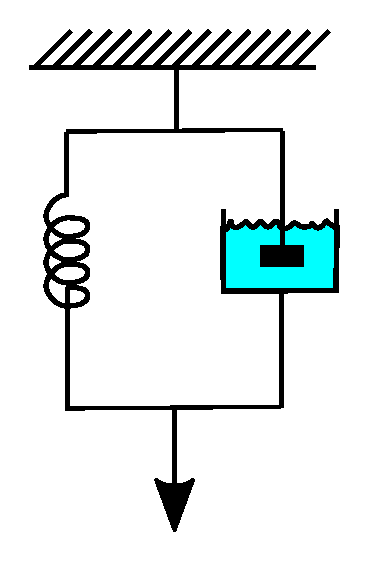
\includegraphics[width=0.25\textwidth]{\figpath/exercises-voigtelement}}
			
			In this case, the total \emph{stress} is the sum of the stresses across the two components, while the total \emph{strain} is identical for each component.
			
			\begin{enumerate}
				\item Express the above statement using appropriate mathematical equations.  Then, find an expression for the total stress in terms of $G_0$, $\eta_0$, and $\gamma$.
				\item Qualitatively, how would you expect the Voigt element to respond to (a) a step strain experiment, and (b) a step stress experiment?  Plot the expected response for each case.
				%\item Find a functional form for the strain, $\gamma(t)$, that results from a step stress of magnitude $\sigma_0$ (note: this is challenging, and requires some knowledge of differential equations).
					%Note: should coach this one more!
			\end{enumerate}
		
\end{exercises}
	
\end{activity}